\section{Fides \& Network Access}
\label{sec:fides-and-network-access}

\begin{figure}[ht]
    \centering
    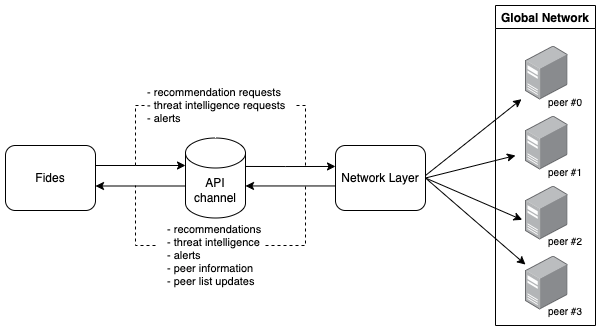
\includegraphics[width=1.0\textwidth]{assets/tl_api_nl.png}
    \caption{Communication between Fides and Network Layer}
    \label{fig:fides-api-network}
\end{figure}

Fides itself is a trust model, set of equations and data storage for interaction history. 
It does not interact with the network directly, bur rather it exposes an API which can be used either to receive the information from the network or for sending the requests back to the network.
Thanks to this design, where all business logic is separated from the network layer, Fides is highly modular and it does not depend on the network layer implementation.
Network layer then performs all data transfers and remote peers communications.
It also facilitates finding new peers and ensuring that all requests from Fides are dispatched to correct recipients.
In the eyes of Fides, network layer is a \textit{blackbox} and it does not need to know, how is the network layer implemented.
See figure \ref{fig:fides-api-network} for high level overview of the communication.

How does the network layer work in detail and what protocols are used describes Martin Řepa in his master's thesis \cite{nl}.